% ------------------------------------------------------------------------------
% TYPO3 Version 10.4 - What's New (Dutch Version)
%
% @license	Creative Commons BY-NC-SA 3.0
% @link		https://typo3.org/help/documentation/whats-new/
% @language	Dutch
% ------------------------------------------------------------------------------

\section{Gebruikersinterface backend}
\begin{frame}[fragile]
	\frametitle{Gebruikersinterface backend}

	\begin{center}\huge{Hoofdstuk 1:}\end{center}
	\begin{center}\huge{\color{typo3darkgrey}\textbf{Gebruikersinterface backend}}\end{center}

\end{frame}

% ------------------------------------------------------------------------------
% ...

\begin{frame}[fragile]
	\frametitle{Gebruikersinterface backend}
	\framesubtitle{Backend UI aanpassingen}

	Kolom met backend-modules heeft een licht gewijzigde UI.

	\begin{figure}
		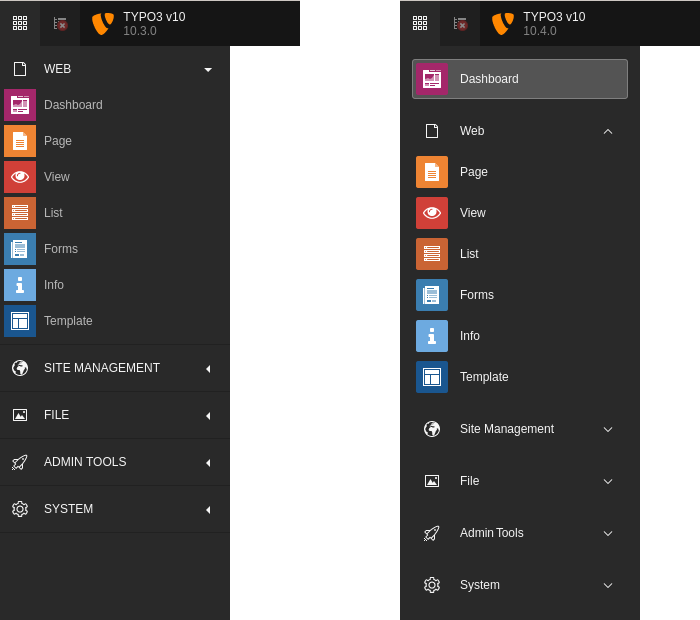
\includegraphics[width=0.5\linewidth]{BackendUserInterface/typo3-backend-ui.png}
	\end{figure}

\end{frame}

% ------------------------------------------------------------------------------
% Feature | 83128 | Content Element Filter

\begin{frame}[fragile]
	\frametitle{Gebruikersinterface backend}
	\framesubtitle{Zoeken nieuw inhoudselement}

	Redacteuren kunnen zoeken naar inhoudselementen in de assistent "Nieuw inhoudselement":

	\begin{figure}
		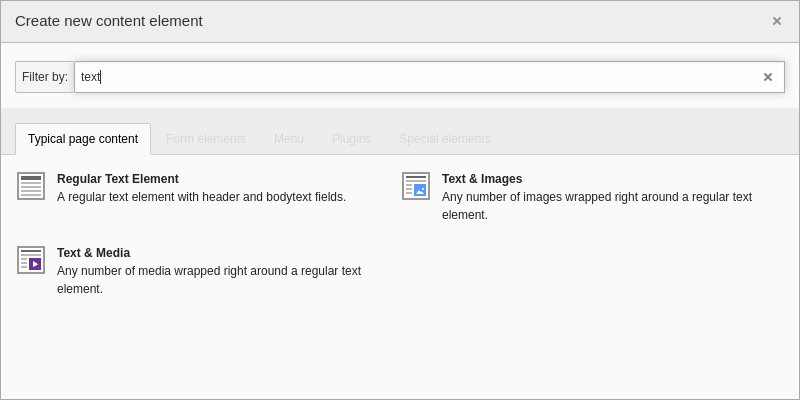
\includegraphics[width=0.6\linewidth]{BackendUserInterface/83128-ContentElementFilter.png}
	\end{figure}

\end{frame}

% ------------------------------------------------------------------------------
% Feature | 89513 | Provide password recovery for backend users

\begin{frame}[fragile]
	\frametitle{Gebruikersinterface backend}
	\framesubtitle{Password Recovery}

	Backend-gebruikers kunnen nu een e-mail vragen voor het herstellen van hun wachtwoord.

	\begin{figure}
		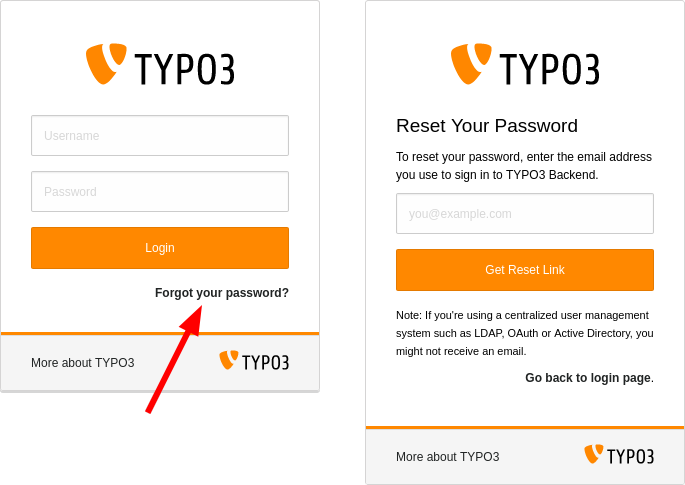
\includegraphics[width=0.6\linewidth]{BackendUserInterface/89513-ProvidePasswordRecoveryForBackendUsers.png}
	\end{figure}

\end{frame}

% ------------------------------------------------------------------------------
